% This is samplepaper.tex, a sample chapter demonstrating the
% LLNCS macro package for Springer Computer Science proceedings;
% Version 2.20 of 2017/10/04
%
\documentclass[runningheads]{llncs}


\usepackage[english]{babel}

% Useful packages
\usepackage[T1]{fontenc}
\usepackage{amsfonts}
\usepackage{amsmath}
\usepackage{amssymb}
\usepackage{graphicx}
\usepackage{hyperref}
\usepackage{verbatim}
\usepackage{cleveref}
\usepackage{xcolor}
\usepackage{tabularx}
\usepackage{booktabs}
\usepackage{lscape}
\usepackage{caption}
\usepackage{subcaption}
\usepackage{xcolor}
\usepackage{ulem}
\usepackage{balance}
\usepackage{booktabs}
\usepackage{multirow}
\usepackage{siunitx}
\usepackage[flushleft]{threeparttable}
\usepackage[justification=centering]{caption}
\sisetup{exponent-product=\cdot,
    retain-explicit-plus,
    retain-zero-exponent}

\def\hide{1}
\renewcommand{\sf}[1]{\textsf{#1}}
\newcommand{\cmark}{\ding{51}}
\newcommand{\xmark}{\ding{55}}
\definecolor{applegreen}{rgb}{0.55, 0.71, 0.0}
\newcommand{\mf}[1]{{\color{applegreen}{#1}}}
\newcommand{\mfc}[2]{\mf{#1} \if\hide1 \sout{\textit{\mf{#2}}} \else \fi}
\newcommand{\mg}[1]{{\color{blue}{\textbf{#1}}}}
\newcommand{\jg}[1]{{\color{orange}{\textbf{#1}}}}
\newcommand{\jgc}[2]{\jg{#1} \if\hide1 \sout{\textit{\jg{#2}}} \else \fi}
\newcommand{\mycomment}[1]{}
\newcommand{\cupdot}{\mathbin{\mathaccent\cdot\cup}}
\DeclareMathOperator*{\argmax}{argmax}


\begin{document}

\sloppy

% \title{AutoClues: AutoML for Clustering Pipelines}
\title{AutoClues: Exploring Clustering Pipelines \\via AutoML and Diversification}


% \author{Anonymous submission}

\author{Matteo Francia\inst{1}\orcidID{0000-0002-0805-1051} \and
Joseph Giovanelli\inst{1}\orcidID{0000-0002-0990-3893} \and
Matteo Golfarelli\inst{1}\orcidID{0000-0002-0437-0725}}

\authorrunning{M. Francia et al.}

\institute{University of Bologna, Cesena, Italy\\
\email{\{m.francia,j.giovanelli,matteo.golfarelli\}@unibo.it}}

\maketitle

\begin{abstract}
AutoML has witnessed effective applications in the field of supervised learning -- mainly in classification tasks --  where the goal is to find the best machine-learning pipeline when a ground truth is available.
This is not the case for unsupervised tasks that are by nature exploratory and they are performed to unveil hidden insights. 
Since there is no right result, analyzing different configurations is more important than returning the best-performing one.
When it comes to exploratory unsupervised tasks -- such as cluster analysis --  different facets of the datasets could be interesting for the data scientist; for instance, data items can be effectively grouped together in different subspaces of features.
In this paper, AutoClues explores and returns a dashboard of both relevant and diverse clusterings via AutoML and diversification.
AutoML ensures that the explored pipelines for cluster analysis (including pre-processing steps) compute good clusterings.
Then, diversification selects, out of the explored clusterings, the ones conveying different clues to the data scientists.
\keywords{AutoML, Clustering, Diversification}
\end{abstract}

\section{Introduction}\label{sec:intro}

\begin{figure}[t]
    \begin{subfigure}[t]{0.23\columnwidth}
        \centering
        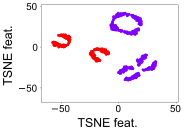
\includegraphics[scale=.15]{img/cl.pdf}
        \caption{Cl \cite{Tschechlov2021}\\ \scriptsize{AMI=0.41, sil=0.41}}
        \label{fig:ca3}
    \end{subfigure}
    ~
    \begin{subfigure}[t]{0.23\columnwidth}
        \centering
        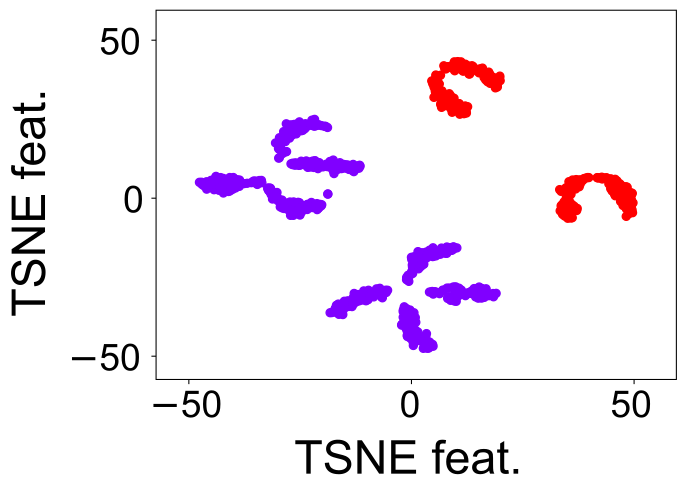
\includegraphics[scale=.15]{img/ft_cl.pdf}
        \caption{FS + Cl\\ \scriptsize{AMI=0.41, sil=0.47}}
        \label{fig:ca4}
    \end{subfigure}
    ~
    \begin{subfigure}[t]{0.2\columnwidth}
        \centering
        \includegraphics[scale=.15]{img/ft_sc_cl.pdf}
        \caption{FS + N + Cl\\ \scriptsize{AMI=0.9, sil=0.87}}
        \label{fig:ca5}
    \end{subfigure}
    ~
    \begin{subfigure}[t]{0.28\columnwidth}
        \centering
        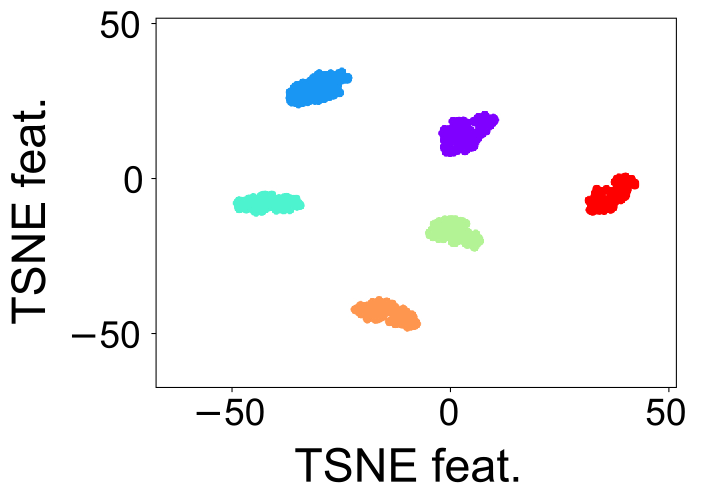
\includegraphics[scale=.15]{img/ft_sc_ou_cl.pdf}
        \caption{FS + N + OR + Cl\\ \scriptsize{AMI=1.0, sil=0.92}}
        \label{fig:ca6}
    \end{subfigure}
    \caption{Approach motivation. \\
    \small{Feature Selection (FS) - Normalization (N) - Outlier Removal (OR) - Clustering (Cl)}}
    \label{fig:clusterings}
\end{figure}

Thanks to the abundant presence of data, machine learning (ML) has been employed in a variety of fields (e.g., urban mobility \cite{toch2019analyzing}).
Depending on the scope of the analysis, the task is defined either supervised (i.e., leveraging a ground truth; e.g., classification) or unsupervised (i.e., without ground truth; e.g., cluster analysis).
Data scientists design the workflow as a \textit{ML pipeline}; namely, a series of pre-processing steps (e.g., features selection) are in charge of shaping the data so that the final analysis step can produce the best result.
For each step of the pipeline, there are alternative algorithms (e.g., SPEC \cite{zhao2007spectral} for feature selection, KMeans \cite{arthur2006k} for cluster analysis), each with hyperparameters to tune (e.g., the number of features or clusters, respectively).

It is well known that, given the exponential search space, the tuning process is tedious and overwhelming.
\textit{Automated Machine Learning} (AutoML) aids in a smart exploration of the hyperparameter search space \cite{hutter2011sequential} and lets data scientists focus on analyzing and interpreting the extracted results.
AutoML has been proven to be effective on supervised tasks where the ground truth eases the evaluation of the hyperparameters optimality   \cite{thornton2013auto,FRANCIA2023182}; yet, when it comes to unsupervised tasks, the road is not paved yet \cite{barlow1989unsupervised}.
In this paper, we focus on the unsupervised task of \textit{(crisp) cluster analysis} \cite{arthur2006k} that returns a partitioning of the original dataset based on the similarity of data items.
Cluster analysis is exploratory by nature since, given that no ground truth is available, there is no ``correct'' result \cite{lensen2017using} and the aim for the data scientist is to uncover clues hidden
in the data.
The two main limitations of the AutoML approaches in the literature are (i) auto-tuning is applied to the ML step only, disregarding the pre-processing ones, and (ii) only the most-performing pipeline configuration is returned; although this is reasonable in the supervised context, it provides limited information in unsupervised one due the exploratory nature of the analysis. 

To overcome the previous limitations, we devise AutoClues: an \textit{end-to-end} AutoML approach that provides a \textit{dashboard} of \textit{relevant} and \textit{different} clusterings. In particular, we focus on the following contributions:
\begin{itemize}
    \item \textit{generalizing} AutoML formulation to deal with unsupervised ML pipelines;
    \item \textit{tuning} a thorough ML pipeline to discover clusterings that would have been unrevealed otherwise;
    \item \textit{diversifying} the generated clusterings to ensure that the dashboard is both high-quality and leads to different insights (i.e., disclose something new);
    \item \textit{providing} a customizable generator of synthetic datasets for benchmarking in (crisp) cluster analysis.
\end{itemize}

To let the reader appreciate the novelty of AutoClues, we rely on a synthetic 10-dimensional (10D) dataset that includes 6 natural clusters. \Cref{fig:ca3} shows the t-SNE \cite{van2008visualizing} visualization\footnote{\textcolor{orange}{This dimensionality reduction visualizes high-dimensional clusterings in 2D, preserving distance proportions. We apply it with the default Scikit-learn hyperparameters.}}  of the clustering obtained applying AutoML4Clust \cite{Tschechlov2021}, an approach of the literature, that solely tunes the clustering step $Cl$. \Cref{fig:ca4,fig:ca5,fig:ca6} show the clusterings obtained by tuning an ML pipeline that incrementally includes feature selection ($FS$), normalization ($N$), and outlier removal ($OR$). In (b), $FS$ identifies the most relevant features; in (c), $N$ standardizes such features thus avoiding bias due to different domain ranges; in (d), $OR$ drops any data items that are not representative. 
It is apparent how the tuning improves throughout the different steps, making it possible for $Cl$ to properly detect the 6 natural clusters. 
To quantitatively understand the improvements, we rely on the silhouette index $sil \in [-1, 1]$ (the higher the better), an estimation of the ``goodness'' of a clustering considering solely the data itself; namely, the \textit{separability} between the clusters and their \textit{cohesion} \cite{zhu2010clustering}.
While in real-case unsupervised problems the ground truth is not available, for our synthetic example we can also measure how the returned clusters match the synthetic ones through the adjusted mutual information \cite{vinh2009information} $AMI \in [0, 1]$ (the higher the better).

\begin{figure}[t]  
    \begin{subfigure}[t]{0.31\columnwidth}
        \centering
        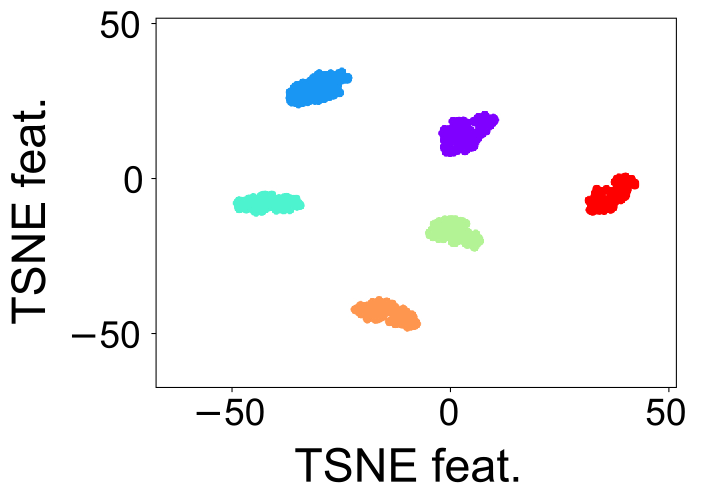
\includegraphics[scale=.15]{img/ft_sc_ou_cl.pdf}
        \caption{FS + N + OR + Cl\\ \scriptsize{AMI=1.0, sil=0.92}}
        \label{fig:d1}
    \end{subfigure}
    ~~
    \begin{subfigure}[t]{0.31\columnwidth}
        \centering
        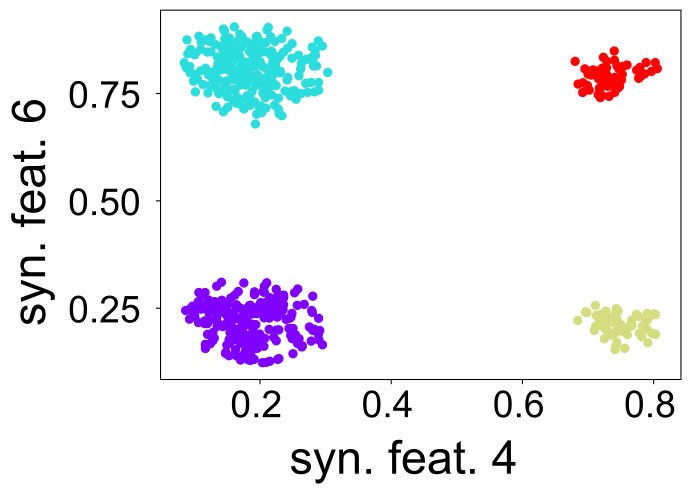
\includegraphics[scale=.15]{img/dashboard_1_pred.pdf}      
        \caption{FS + OR + Cl\\ \scriptsize{AMI=0.65, sil=0.86}}
        \label{fig:d3}
    \end{subfigure}
    ~
    \begin{subfigure}[t]{0.31\columnwidth}
        \centering
        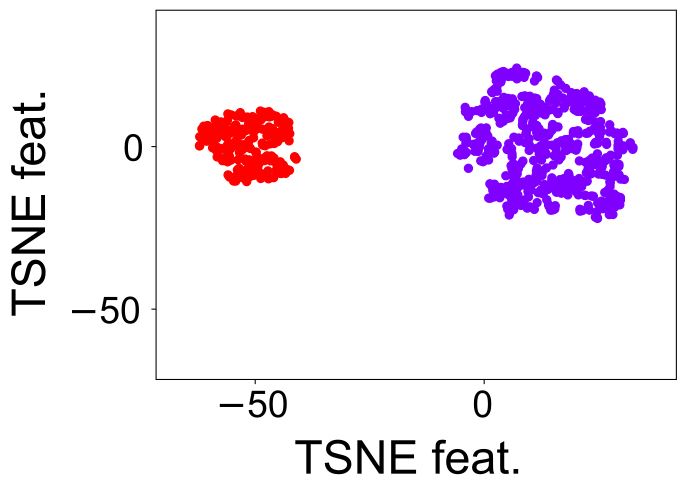
\includegraphics[scale=.15]{img/dashboard_2_pred.pdf}  
        \caption{FS + OR + Cl\\ \scriptsize{AMI=0.38, sil=0.74}}
        \label{fig:d2}
    \end{subfigure}
    \caption{Relevant and diverse clusterings returned by AutoClues.\\
    \small{Feature Selection (FS) - Normalization (N) - Outlier Removal (OR) - Clustering (Cl)}}
    \label{fig:dashboard}
\end{figure}

As to the limitation of returning only the most-performing pipeline configuration, \Cref{fig:dashboard} depicts an example of an AutoClues dashboard with three different facets (clustering).
Along with the expected clusters (a), the representation in (b) unveils 4 macro clusters in 2 original features, while the representation in (c) highlights a large gap of 2 main clusters.
In real-world problems, those facets may help the data scientist to understand the data.
% by providing different interpretations of their semantics.

% We organize the paper as follows.
% \Cref{sec:related} discusses the related contributions.
% \Cref{sec:autoclues} introduces the problem formulation and how AutoClues tackles it.
% \Cref{sec:test} illustrates the benchmark generator and dives into the empirical evaluation of the approach. Finally,  \Cref{sec:conclusion} draws the conclusion and future research directions.

\section{Related works}\label{sec:related}

Although the active development of data pre-processing techniques in cluster analysis (e.g., outlier removal, feature selection), and the evidence of their benefits, there is no trace of automatic solutions that tunes a thorough ML pipeline.

Former approaches employed model-free techniques (i.e., without a model to drive the optimization) to tune the combination of number of clusters and number of features.
Evolutionary algorithms are population-based heuristics inspired by biological evolution mechanisms (e.g., reproduction, mutation) or physical phenomena (e.g., particle swarm, black holes).
The population is intended as the search space, individuals are configurations, and a mutation mechanism allows the modification of the current candidate, hence the exploration.
Recent works that follow this modus operandi (i.e., MOGA \cite{dutta2013}, MODE-cf \cite{hancer2020new}, \textcolor{orange}{TPE-AutoClust \cite{10031132}}) compose the candidate with a string that encodes information about both the feature selection and the clustering.
Authors in \cite{simulate_annealing} leverage simulated annealing, an algorithm that comes from a technique involving heating and controlled cooling of material in metallurgy.
In \cite{prakash2019gravitational}, it is leveraged a gravitational search algorithm, inspired by the theory of Newtonian gravity.

Model-based techniques leverage past evaluations to fit a model and visit the most prominent configurations.
Such techniques have been proven to achieve extremely good results, specifically in the (supervised) AutoML field where a pipeline has to be instantiated with different algorithms and hyperparameters.
Authors in \cite{Tschechlov2021,poulakis2020autoclust,Liu2021} apply such techniques on cluster analysis, but do not consider any pre-processing phase.
In MALSS \cite{Kamoshida2020}, the authors apply AutoML with simple (no-clustering-oriented) pre-processing, and still for the aim of suggesting the number of clusters.
\textcolor{orange}{In \cite{ENES20231}, authors introduce a pipeline for unsupervised clustering, yet specifically tailored for multivariate time series originating from HPC job monitoring.}
Finally, such approaches retrieve just one solution.

\section{AutoClues}\label{sec:autoclues}

\begin{figure}[t]
    \centering
    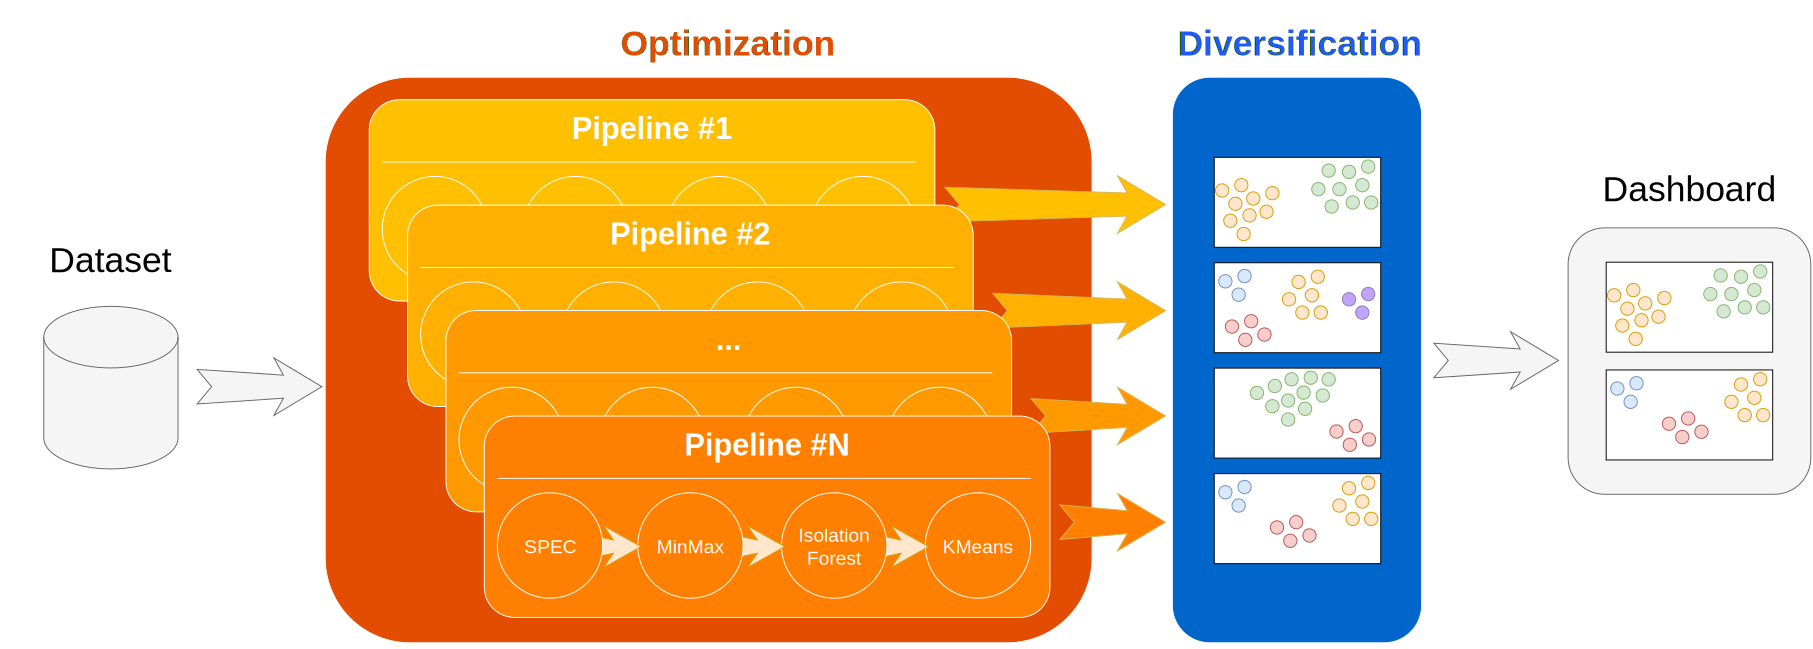
\includegraphics[scale=.26]{img/approach.pdf}
    \caption{Overview of AutoClues.}
    \label{fig:overview}
\end{figure}

AutoClues aims at (i) tuning the whole ML pipeline and (ii) suggesting multiple clusterings to provide the data scientist different facets of the datasets. 
In literature, these two problems are addressed through \textit{optimization} and \textit{diversification} techniques respectively.
\Cref{fig:overview} shows an overview of the architecture.

\subsection{Formalization}
\label{ssec:formalization}

\textbf{Optimization} We seek for the most ``correct'' pipeline.
A pipeline is a sequence of steps that process a dataset in order to return a clustering and, at each step, an algorithm can be picked among several alternatives.

More formally, a \textit{dataset} $D$ is a collection of $|D|$ data items that is characterized by a set of features $\mathcal{F}$ (i.e., columns).
An \textit{Algorithm} $A$ is a function that transforms a dataset $D'$ into a new dataset $D''$ and has a set of (possibly empty) \textit{hyperparameters} that regulates its behavior.
Each hyperparameter has a domain, and the possible algorithm configurations are represented as the Cartesian product of all the hyperparameter domains, denoted with $\Lambda_A$.
We call \textit{algorithm instance} $\lambda_A \in \Lambda_A$ an (ordered) tuple in which each hyperparameter has been assigned with a value from its domain.
For instance, a clustering algorithm is KMeans and two tunable hyperparameters can be: the number of clusters $k \in \mathbb{N}^+$ and the maximum iterations $iter \in \mathbb{N}^+$. 

A pipeline \textit{step} $S$ is a set of algorithms that can be selected as alternatives to carry out the step goal, including the possibility to return the dataset as-is through the ``Identity'' algorithm $I$.
%
The step domain is defined as $\Lambda_S = \Lambda_{A_1} \cupdot \ldots \cupdot \Lambda_{A_{|S|}}$, therefore the disjoint union of the domain of each algorithm\footnote{If an algorithm has no hyperparameters ($\Lambda_{A} = \varnothing$), we set a placeholder $\Lambda_{A} = \{ 1 \}$.}. $\lambda_{S}$ denotes the algorithm instance selected for the step.

A \textit{Pipeline} $P$ is a sequence of steps, its domain is the Cartesian Product of the step domains $\Lambda_P = \Lambda_{S_1} \times \ldots \times \Lambda_{S_{|P|}}$, and a \textit{pipeline instance} is an ordered tuple of algorithm instances $\lambda_P = (\lambda_{S_1}, \ldots, \lambda_{S_{|P|}}) \in \Lambda_P$.
The input of $\lambda_{A_i}$ is the output of $\lambda_{A_{i-1}}$ and the initial dataset $D$ is the input of $\lambda_{A_{1}}$.
In our use case, the last step is mandatory since it fulfills cluster analysis by returning a clustering.

A \textit{(crisp) Clustering} is a partition of the dataset into a set of non-overlapping clusters  $C=\{c_1, \ldots, c_{|C|}\}$ (i.e., groups of data items) by minimizing the distance of data items in the same cluster and maximizing the distance of different clusters. 
Given a pipeline domain $\Lambda_P$ and a dataset $D$, the optimal instance is 
\begin{equation}
\label{eq:optimization}
    \lambda_P^* = argmax_{\lambda_P \in \Lambda_P} rel(C)
\end{equation}
where $rel$ is a goodness metric for $C$ obtained by applying $\lambda_P$ on $D$.
\\
\\
\textbf{Diversification} The process of returning a set of relevant and diverse solutions -- clusterings in our case -- is known as diversification, a multi-objective optimization problem that can be formulated as follows.
%
Let $\mathcal{C}$ be the set of clusterings that have been explored in the pipeline optimization process (\Cref{eq:optimization}), then our goal is selecting a set of $\alpha$ clusterings $\mathcal{C}^* \subseteq \mathcal{C}$ maximizing a \textit{score} that represents a tradeoff between finding \textit{relevance} and \textit{diversity}.
%
\begin{align}\label{def:score}
&\mathcal{C}^* = argmax_{\hat{\mathcal{C}} \subseteq \mathcal{C}, \alpha=|\hat{\mathcal{C}}|} score(\beta, \hat{\mathcal{C}})\\
&score(\beta, \hat{\mathcal{C}}) = (1-\beta)~rel(\hat{\mathcal{C}}) + \beta~div(\hat{\mathcal{C}})
\end{align}
where $\beta \in [0.. 1]$ is the tradeoff parameter and
\begin{align}
rel(\hat{\mathcal{C}}) &= (|\hat{\mathcal{C}}|-1)\sum_{C \in \hat{\mathcal{C}}} rel(C)
\label{def:rel}
\end{align}
\begin{align}
div(\hat{\mathcal{C}}) &= \sum_{C_i \in \hat{\mathcal{C}}}~\sum_{C_j \in (\hat{\mathcal{C}} \setminus C_i)} div(C_i, C_j)
\label{def:div}
\end{align}

\noindent $div(\hat{\mathcal{C}})$ is the sum of pairwise clustering diversity comparisons and $rel(\hat{\mathcal{C}})$ is the sum of clustering relevance;
$rel(\hat{\mathcal{C}})$ entails a multiplication factor $|\hat{\mathcal{C}}|-1$ to make $rel(\hat{\mathcal{C}})$ and $div(\hat{\mathcal{C}})$ comparable.

\subsection{Implementation}\label{sec:implementation}

\begin{table}[t]
    \centering
    \begin{tabular}{llcc}
        \hline
        Step     & Algorithm & \#Hyper. & $|\Lambda_A|$\\\hline
        Feature selection & SPEC \cite{zhao2007spectral} & 1 & $|\mathcal{F}|-1$\\
         & WKMeans \cite{WKMeans} & 2 & $3 \cdot (|\mathcal{F}|-1)$\\
         & Pearson Filtering & 1 & 10\\
        Normalization     & Standardization & 0 & 1\\
        & Robust Scaling & 3 & 12\\
        & MinMax & 0 & 1\\
        Outlier removal   & Local Outlier Factor \cite{breunig2000lof} & 1 & 3\\
        & Isolation Forest \cite{liu2012isolation} & 1 & 3\\
        %Cluster analysis  & KMeans \cite{arthur2006k} & $n \in [2.. \frac{|D|}{2}]$ \\
        Clustering  & KMeans \cite{arthur2006k} & 1 & $\sqrt{|D|}$\\
        & Agglomerative clustering  \cite{murtagh2017algorithms} & 1 & $\sqrt{|D|}$\\\hline
    \end{tabular}
    \caption{Steps and algorithms optimized by AutoClues.}
    \label{tbl:processing}
\end{table}


\Cref{tbl:processing} reports the pipeline with steps, algorithms, and hyperparameters; AutoClues is available on GitHub \footnote{\url{https://github.com/big-unibo/autoclues}}.
The first step is \textit{Feature selection}. 
Since cluster analysis is particularly sensitive to non-informative and correlated features, we leverage algorithms from spectral family and based on the Pearson correlation, respectively. 
Follows, \textit{Normalization} to adjust values on different scales and ensure that all the features contribute equally to the cluster formation.
Here, the literature has a considerable consensus on the well-known techniques such as Standardization, Robust scaling, and Min-max.
The last pre-processing step is \textit{Outlier Removal} for discarding any data points that are not representative of the cluster, we leverage Local Outlier Factor \cite{breunig2000lof} and and Isolation Forest \cite{liu2012isolation}.
Finally, the \textit{Clustering} step.
Since we focus on \textit{crisp spherical} clustering algorithms, we consider KMeans \cite{arthur2006k} and Agglomerative Clustering \cite{murtagh2017algorithms} with complete linkage.
As to the order of steps, in \cite{giovanelli2022data}, the authors reduce the combinations of the former steps; we further constrained the order of the steps by computing several experiments and observing the impact of the alternatives.
\\
\\
\textbf{Optimization}
To explore promising pipeline instances, we leverage Bayesian Optimization (BO) \cite{hutter2011sequential}.
BO is iterative: as it explores hyperparameter configurations, it progressively builds an accurate model of the domain to decide the next configuration to explore.
The exploration continues until a budget in terms of either iterations or time is reached.

Selecting the optimal pipeline instance requires the relevance metric (i.e., $rel(C)$) to evaluate the goodness of the retrieved clustering.
In AutoClues, such a metric is customizable.
Well-known metrics leveraged for spherical clustering are: the silhouette index (SIL) \cite{zhu2010clustering}, contrasting the average distance to elements in the same cluster with the average distance to elements in other clusters, and the Davies-Bouldin Index (DBI) \cite{dbi}, computing the average similarity between clusters by considering their own size.
However, clustering metrics show a bias toward lower dimensionalities i.e., yielding higher scores when fewer features are chosen \cite{lensen2017using,hancer2020new}. 
\textcolor{orange}{To overcome this, we employ t-SNE \cite{van2008visualizing} (with default Scikit-learn hyperparameters) to project the clusterings to a latent 2D space.
Distances in this latent space are preserved, and we can compute the chosen metric atop,  enabling a fair evaluation of clusterings across diverse feature spaces.}
%
% During the optimization, we also store the computed pipeline instances since our goal is returning diverse and relevant clusterings.
\\
\\
\textbf{Diversification}
Implementing diversification in cluster analysis involves assessing the extent to which two clusterings differ from each other, hence how the returned dashboard looks.
It is crucial to rely on a metric that considers not only shared cluster membership but also structural interrelationships.

Information theory introduces the concept of Mutual Information, quantifying the degree of dependence between two variables and, more specifically, Adjusted Mutual Information (AMI) allows for chance agreement\footnote{In statistics, it serves as a baseline for assessing the significance in random variations.}---providing more robust and meaningful measures.
When applied to cluster analysis, AMI $\in [0, 1]$ considers the labels assigned to data points within clusters, assuming higher values when the clusters in one partition align with those in another.
Since we need a diversity metric, we adapt the formula as in:
$$div(C_i, C_j) = 1- AMI(C_i, C_j)$$ 
where $C_i, C_j$ clusterings coming from different pipeline instances.

Finally, considering that the diversification problem is NP-hard, we compute it by exploiting the MMR heuristic solution\footnote{\textcolor{orange}{We use the default hyperparameter $\beta = 0.5$, and set $\alpha$ according to the test at hand.}} \cite{vieira2011query} that selects the best-performing clustering and iteratively adds the clusterings that most diversify the outcome.

\section{Benchmark Generation and Empirical Evaluation}\label{sec:test}


\begin{table}[t]
    \centering
    \footnotesize
    \begin{tabular}{l|ccccccc|cccc}
    \hline
        \multirow{2}{*}{Dataset}& \multicolumn{7}{c|}{Characteristics} & \multicolumn{4}{c}{AutoClues Performance} \\
        & $|D|$ & $|\mathcal{F}|$ & $|\mathcal{C}|$ & $\sigma(D)$ & $\sigma(\mathcal{F})$ & $SIL_N$ & $SIL_B$ & $SIL$ & $AMI$ & Score & Div. time (s) \\ \hline
         \texttt{syn1} & 2905 & 2  & 3 & 0.15  & 0.50  & 0.72 & 0.48 & 0.79 & 1.0 & 4.12 & \num{1.64e03} \\ 
        \texttt{syn2} & 264 & 5  & 3 & 0.25  & 0.20  & 0.64 & 0.4 & 0.7 & 0.83 & 4.76 & \num{1.74e02} \\ 
        \texttt{syn3} & 900 & 7  & 12 & 0.11  & 0.14  & 0.88 & 0.6 & 0.92 & 1.0 & 4.39 & \num{1.51e03} \\ 
        \texttt{syn4} & 1446 & 2  & 13 & 0.22  & 1.00  & 0.59 & 0.31 & 0.85 & 0.95 & 3.92 & \num{2.99e03} \\ 
        \texttt{syn5} & 1673 & 4  & 8 & 0.17  & 0.25  & 0.71 & 0.54 & 0.81 & 0.99 & 4.22 & \num{2.18e03} \\ 
        \texttt{syn6} & 2905 & 2  & 3 & 0.15  & 0.50  & 0.72 & 0.61 & 0.84 & 0.87 & 4.63 & \num{1.07e03} \\ 
        \texttt{syn7} & 264 & 5  & 3 & 0.25  & 0.20  & 0.64 & 0.41 & 0.72 & 0.86 & 3.78 & \num{1.67e02} \\ 
        \texttt{syn8} & 1639 & 8  & 21 & 0.13  & 0.00  & 0.87 & 0.69 & 0.91 & 1.0 & 4.45 & \num{3.13e03} \\ 
        \texttt{syn9} & 525 & 3  & 2 & 0.21  & 0.00  & 0.66 & 0.42 & 0.69 & 0.87 & 3.96 & \num{3.67e02} \\ 
        \texttt{syn10} & 1446 & 2  & 13 & 0.22  & 1.00  & 0.59 & 0.32 & 0.86 & 0.97 & 4.03 & \num{4.09e03} \\ 
        \texttt{syn11} & 4813 & 10  & 3 & 0.27  & 0.40  & 0.46 & 0.17 & 0.09 & 0.42 & 2.92 & \num{1.08e02} \\ 
        \texttt{syn12} & 2905 & 2  & 3 & 0.15  & 0.50  & 0.72 & 0.57 & 0.79 & 1.0 & 4.48 & \num{1.62e03} \\ 
        \texttt{syn13} & 264 & 5  & 3 & 0.25  & 0.20  & 0.64 & 0.4 & 0.74 & 0.89 & 4.37 & \num{2.75e02} \\ 
        \texttt{syn14} & 525 & 3  & 2 & 0.21  & 0.00  & 0.66 & 0.22 & 0.71 & 0.9 & 4.38 & \num{5.81e02} \\ 
        \texttt{syn15} & 2905 & 2  & 3 & 0.15  & 0.50  & 0.72 & 0.61 & 0.81 & 1.0 & 4.06 & \num{1.13e03} \\ 
        \texttt{syn16} & 264 & 5  & 3 & 0.25  & 0.20  & 0.64 & 0.49 & 0.7 & 0.88 & 3.45 & \num{1.84e02} \\ 
        \texttt{syn17} & 900 & 7  & 12 & 0.11  & 0.14  & 0.88 & 0.41 & 0.92 & 1.0 & 4.62 & \num{1.45e03} \\ 
        \texttt{syn18} & 525 & 3  & 2 & 0.21  & 0.00  & 0.66 & 0.3 & 0.69 & 0.84 & 4.34 & \num{2.85e02} \\ 
        \texttt{syn19} & 2905 & 2  & 3 & 0.15  & 0.50  & 0.72 & 0.53 & 0.86 & 0.87 & 4.79 & \num{1.28e03} \\ 
        \texttt{syn20} & 264 & 5 & 3 & 0.25 & 0.20 & 0.64 & 0.44 & 0.7 & 0.88 & 3.74 & \num{2.13e02} \\ \hline
    \end{tabular}
    % \vspace{0.2cm}
    \caption{Dataset characteristics and performance achieved by AutoClues.}
    \label{tbl:synthetic}
\end{table}

Evaluation in cluster analysis consists of assessing the approach performance in finding well-separated clusters and -- if available -- their alignment with a hypothetical ground truth.
It is crucial to test on datasets that conform with the leveraged clustering algorithms, e.g., in our case, containing crisp spherical clusters.
Yet, there is a lack of benchmarks (i.e., suites of datasets for fair comparisons) and the few available \cite{ClusteringDatasets,gagolewski2022framework,thrun2020clustering} are tailored to their specific scenarios.
This translates into approaches relying upon datasets from supervised tasks, with no guarantees on the underlying clusters' shape.
% Cluster analysis lacks benchmark availability i.e., suites of datasets for fair comparisons, mainly due to the large number of clustering families (e.g., crisp, fuzzy) and cluster shapes (e.g., spherical, worm). Existing benchmarks \cite{ClusteringDatasets,gagolewski2022framework,thrun2020clustering} are tailored to their specific scenarios, leading cases as ours to the reliance on datasets from supervised tasks. 
% Yet, with no guarantees on the underlying clusters' shape, comprehensive evaluations remain challenging.

In \Cref{ssec:benchmark}, we introduce a benchmarking generator and a suite of synthetic datasets. In \Cref{ssec:effectiveness}, we leverage such a suite to assess the effectiveness and efficiency of AutoClues.
Finally, in \Cref{ssec:comparison}, we rely on real datasets to provide a comparison against other approaches in the literature.

\subsection{Benchmark Generation}
\label{ssec:benchmark}
The synthetic benchmarking generator is available at \url{https:/github.com/big-unibo/clustering_benchmarking}.
We create datasets of $|D|$ instances, defining $|C|$ natural hyper-spherical clusters in a space of $|\mathcal{F}|$ features.
Then, we blur such clusters by posing common challenges faced by clustering algorithms. 
This includes noise on instances $\sigma(D)$, such as the presence of outliers, and
noise on features $\sigma(F)$, such as irrelevant, correlated, or distorted features.

To obtain datasets with different characteristics, we set boundaries for each of these dimensions and sample within them according to the Sobol sequence \cite{sobol1967distribution}, a quasi-random low-discrepancy search converging to an equi-distributed coverage. 
In particular, the defined boundaries are: $|D|$ between $100$ and $5000$, $|F|$ between $2$ and $10$, $|C|$ between $2$ and $\sqrt{|D|}$, $\sigma(D)$ between $0.1$ and $0.3$, and $\sigma(F)$ between $0$ and $1$.
\Cref{tbl:synthetic} provides a suite of $20$ synthetic datasets. 

Dataset complexity can be examined via the silhouette $SIL \in [0, 1]$, the higher the simpler. 
$SIL_N$ measures the cohesion and separability of the natural clusters $C$ in their original feature space, while  $SIL_B$ measures the silhouette of blurred clusters (i.e. after introducing noise ($\sigma$)).
The former $SIL_N$ indicates the presence of well-separated clusters.
With the first quartile $Q1=0.64$, median $Q2=0.66$, and third quartile $Q3=0.72$, we observe that 25\% of datasets are complex already at this stage. 
The latter $SIL_B$ registers significantly lower values: \texttt{syn11} emerges as an especially complex dataset with $SIL_B=0.17$ but, overall, we confirm the presence of a good distribution between more and less challenging datasets: $Q1 = 0.36$, $Q2 = 0.43$, and $Q3 = 0.55$.

\subsection{Effectiveness and efficiency}
\label{ssec:effectiveness}


We test AutoClues on the suite of generated synthetic datasets.
For the optimization, we adopted the silhouette $SIL$ index as a relevance objective metric and a budget of $7200$ seconds ($2$ hours); for the diversification we set $\alpha=3$ and $\beta=0.5$, resulting in a dashboard of $3$ clusterings where relevance and diversity are weighted equally.
Tests are run on a single core of an Intel Core i7 machine at $3.20$ GHz and $64$ GB of main memory.
%
Given an AutoClues dashboard, \Cref{tbl:synthetic} provides
the maximum $SIL\in [0, 1]$ as the cohesion of the found clusters and the maximum $AMI \in [0, 1]$ as the alignment with the natural ones\footnote{\textcolor{orange}{Metrics are computed on the original dataset (i.e., no t-SNE distortion)}}. Besides, we report the dashboard score of \Cref{def:score}, summarizing the overall relevance and diversity in the dashboard, and the diversification computation time.
\\
\\
\textbf{Effectiveness}
The achieved silhouette not only shows AutoClues' ability to find well-separated clusters in 19 cases out of 20, but it also demonstrates to overcome the silhouette of natural clusters $SIL_N$. 
This is achieved through pre-processing such as projecting natural clusters into more compact feature subsets and mitigating potential noise.
The only critical exception is \texttt{syn11}, already highlighted in the previous section. 
$AMI$ also confirms strong agreement between retrieved and natural clusters ($Q1=0.87$, $Q2=0.9$, $Q3=1$). 

As to the dashboard, considering the experimental setting ($\alpha=3$, $\beta=0.5$,  $rel, div \in [0, 1]$), the score is bounded in $[0, 6]$.
Notably, given the inherent trade-off relationship between \textit{rel} and \textit{div} in the context of a diversification problem, it is noteworthy that scores at the boundaries are less likely to manifest,
with values around $4$ already acknowledged as high-quality \cite{vieira2011query}.
Analogously, quartile values of the score ($Q1=4$, $Q2=4.34$, $Q3=4.47$) confirm Autoclues' ability to find relevant and diverse clusterings.
\\
\\
\textbf{Efficiency}
\Cref{tbl:synthetic} reports the computation time for diversification, when the optimization budget is set to 2 hours.
We can observe 25\% of datasets compute the dashboard in less than $Q1=\num{2.44e02}$ seconds ($4$ minutes), $50\%$ in less than $Q2=\num{1.07e03}$ seconds ($18$ minutes), and $75\%$ in less than $Q3=\num{1.56e03}$ seconds ($26$ minutes).
Besides, reducing the optimization budget leads to a decrease in diversification time, maintaining high performance.
%
\Cref{fig:convergence} shows how AutoClues converges to the values reported in \Cref{tbl:synthetic}.
Dashboards are generated at different snapshots during the $2$-hour optimization process, and the same metrics are computed: $SIL$, $AMI$, dashboard score, and diversification time.
We summarize the information by plotting the mean and standard deviation among the whole suite, the convergence is quantified as a progress ratio relative to the final achieved performance.
Notably, the optimization time is illustrated in a logarithmic scale, highlighting already fast convergence.
After $60$ seconds of optimization, we have clusterings with $SIL$ and $AMI$ as good as $80\%$ and $95\%$ of the optimal and a dashboard almost $60\%$ of the final within a negligible diversification time---roughly $2\%$ of the total, $30$ seconds on average.

\begin{figure}[t]
    \centering
    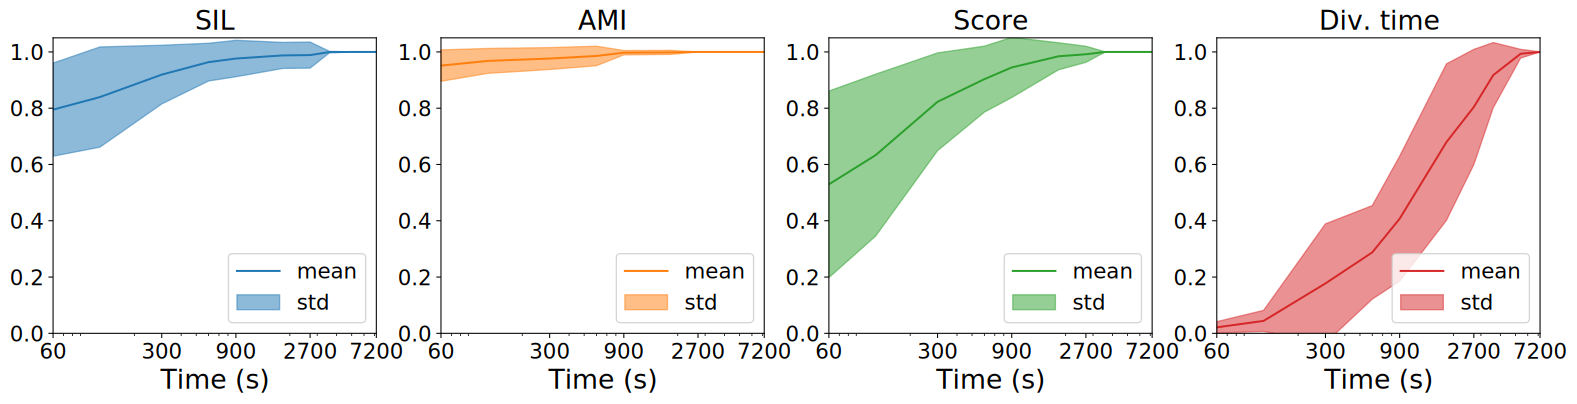
\includegraphics[scale=.3]{img/all.pdf}
    \caption{AutoClues convergence through time (in log scale).}
    \label{fig:convergence}
\end{figure}

Within $300$ seconds of optimization, an average of $90\%$ of $SIL$, $97\%$ of $AMI$, and $75\%$ of the dashboard score are registered with a diversification cost of $10\%$---on average, $1$ minute and half.
The trends of $SIL$ and $AMI$ saturated $100\%$ right afterward, while both dashboard score and cost increase linearly until $900$ seconds of optimization, in which the dashboard achieves $90\%$ of its score within a cost of $30\%$---$5$ minutes on average.
After such a threshold, improvements in the score are not considered worth it for the computation cost.
This is due to the increasing number of solutions to be evaluated during diversification, while relevant and diverse clusterings are already present in the dashboard.

\subsection{Comparison}\label{ssec:comparison}

\begin{table}[t]
    \centering
    \begin{tabular}{l|ccc|cccc|cc}
    \hline
        \multirow{3}{*}{Dataset} & \multicolumn{3}{c|}{Characteristics} & \multicolumn{6}{c}{Performance} \\
        & \multirow{2}{*}{$|D|$} & \multirow{2}{*}{$|\mathcal{F}|$} & \multirow{2}{*}{$|C|$} & \multicolumn{4}{c|}{DBI $\downarrow$} & \multicolumn{2}{c}{SIL $\uparrow$} \\
        & & & & \multicolumn{1}{c}{MOGA} & \multicolumn{1}{c}{MODE-cf} & \multicolumn{1}{c}{MALSS} & \multicolumn{1}{c|}{AutoClues} & \multicolumn{1}{c}{MALSS} & \multicolumn{1}{c}{AutoClues} \\ \hline
        \texttt{blood} & 748 & 4 & 2 & - & - & 0.3 & \textbf{0} & 0.73 & \textbf{1} \\ 
        \texttt{breast} & 106 & 9 & 6 & - & 0.7 & 1.6 & \textbf{0.54} & 0.16 & \textbf{0.60} \\ 
        \texttt{ecoli} & 327 & 7 & 5 & - & 0.92 & \textbf{0.35} & 0.46 & \textbf{0.72} & 0.46 \\ 
        \texttt{iris} & 150 & 4 & 3 & 0.39 & 0.67 & 0.6 & \textbf{0.38} & 0.57 & \textbf{0.71} \\
        \texttt{seeds} & 210 & 7 & 3 & - & - & 0.8 & \textbf{0.4} & \textbf{0.45} & 0.37 \\
        \texttt{thyroid} & 215 & 5 & 3 & - & - & 0.64 & \textbf{0.2} & 0.6 & \textbf{0.92} \\ 
        \texttt{vehicle} & 846 & 18 & 4 & - & - & 0.6 & \textbf{0.15} & 0.61 & \textbf{0.72} \\ 
        \texttt{wine} & 178 & 13 & 3 & \textbf{0.77} & 1.22 & 1.4 & 1.01 & 0.28 & \textbf{0.38} \\ \hline
    \end{tabular}
    % \vspace{0.2cm}
    \caption{Comparison with other approaches in the literature.}
    \label{tbl:comparison}
\end{table}


We compare AutoClues with state-of-the-art approaches in the literature against real datasets, considered as standard benchmarks.
We selected the ones that provided either the performance on classification datasets (MOGA \cite{dutta2013}, MODE-cf \cite{hancer2020new}) or code for reproducibility (MALSS \cite{Kamoshida2020}).
The former two approaches are evolutionary algorithms, and the latter is a general-purpose AutoML tool.
These approaches do not provide a dashboard but only the best-performing clustering.
Thus, for a fair comparison, we set $\alpha=1$ to return the best clustering, and we adopt as relevance the same metric used in the competing approaches.
MOGA and MODE-cf measure performance solely through the Davies–Bouldin Index ($DBI$ \cite{dbi}, the less the better),
MALLS also provides $SIL$ (the higher the better).

\Cref{tbl:comparison} shows that AutoClues outperforms the reported approaches in 6 out of 8 datasets.
According to $DBI$, MALSS achieves better performance on \texttt{seeds}, while MOGA on \texttt{wine}.
As to $SIL$, MALSS is slightly more performant in \texttt{ecoli} and \texttt{seeds}.
Yet, this is due to the fact that such approaches support the computation of non-spherical clusterings while they are not currently included in AutoClues. 
Indeed, if we constraint MALSS to compute spherical clusters only, we observe a $DBI$ value of $0.79$ for \texttt{ecoli} while AutoClues achieves $0.46$ (the less the better).
As to $SIL$, MALLS achieves $0.4$ and $0.45$ for \texttt{ecoli} and \texttt{seeds} respectively; AutoClues outperforms on \texttt{ecoli} with $SIL=0.46$ and confirms the previous result on \texttt{seeds} with $SIL=0.37$.

\section{Conclusion and Future Work}\label{sec:conclusion}
We introduced AutoClues, an end-to-end cluster analysis approach that leverages AutoML techniques to provide a diverse and relevant dashboard of clusterings. Our findings demonstrate that optimizing pre-processing significantly enhances performance, allowing AutoClues to overcome current state-of-the-art approaches. For future research, we plan to explore (i) meta-learning approaches to identify more effective pre-processing steps, (ii) integrating human feedback in the loop, and (iii) providing automatic explanations for the retrieved dashboard.

\bibliographystyle{splncs04}
\bibliography{refs}


\end{document}
